% ============================================
% Chapitre 4 : Déploiement Zabbix avec Docker
% ============================================
\chapter{Déploiement du Serveur Zabbix}
\label{chap:zabbix-deployment}

\section{Installation de Docker}

\subsection{Mise à jour du Système}

Après connexion au serveur Zabbix via SSH, la première étape consiste à mettre à jour le système :

\begin{lstlisting}[language=bash, caption=Mise à jour du système]
sudo apt update && sudo apt upgrade -y
\end{lstlisting}

\subsection{Installation de Docker Engine}

Installation de Docker et Docker Compose :

\begin{lstlisting}[language=bash, caption=Installation de Docker]
# Installation des prerequis
sudo apt install -y ca-certificates curl gnupg

# Ajout de la cle GPG Docker
sudo install -m 0755 -d /etc/apt/keyrings
curl -fsSL https://download.docker.com/linux/ubuntu/gpg | \
    sudo gpg --dearmor -o /etc/apt/keyrings/docker.gpg

# Ajout du repository Docker
echo "deb [arch=$(dpkg --print-architecture) \
    signed-by=/etc/apt/keyrings/docker.gpg] \
    https://download.docker.com/linux/ubuntu \
    $(lsb_release -cs) stable" | \
    sudo tee /etc/apt/sources.list.d/docker.list

# Installation de Docker
sudo apt update
sudo apt install -y docker-ce docker-ce-cli \
    containerd.io docker-compose-plugin

# Ajout de l'utilisateur au groupe docker
sudo usermod -aG docker $USER
\end{lstlisting}

\begin{figure}[H]
\centering

\includegraphics[width=0.95\textwidth]{images/15-docker-installation.png}
\caption{Installation de Docker réussie}
\label{fig:docker-installation}
\end{figure}

\subsection{Vérification de l'Installation}

\begin{lstlisting}[language=bash, caption=Vérification de Docker]
docker --version
docker compose version
\end{lstlisting}

\section{Configuration de Zabbix}

\subsection{Création du Fichier docker-compose.yml}

Le fichier docker-compose.yml définit l'ensemble de la stack Zabbix :

\begin{lstlisting}[language=bash, caption=Création du répertoire et du fichier]
mkdir ~/zabbix && cd ~/zabbix
nano docker-compose.yml
\end{lstlisting}

\begin{lstlisting}[caption=Contenu du docker-compose.yml, label=lst:docker-compose]
version: "3.8"

services:
  # Base de donnees MySQL
  mysql-server:
    image: mysql:8.0
    container_name: zabbix-mysql
    restart: always
    environment:
      MYSQL_DATABASE: zabbix
      MYSQL_USER: zabbix
      MYSQL_PASSWORD: zabbix_pwd_secure
      MYSQL_ROOT_PASSWORD: root_pwd_secure
    command:
      - mysqld
      - --character-set-server=utf8mb4
      - --collation-server=utf8mb4_bin
    volumes:
      - mysql_data:/var/lib/mysql
    networks:
      - zabbix-net

  # Serveur Zabbix
  zabbix-server:
    image: zabbix/zabbix-server-mysql:alpine-7.0-latest
    container_name: zabbix-server
    restart: always
    environment:
      DB_SERVER_HOST: mysql-server
      MYSQL_DATABASE: zabbix
      MYSQL_USER: zabbix
      MYSQL_PASSWORD: zabbix_pwd_secure
    ports:
      - "10051:10051"
    depends_on:
      - mysql-server
    networks:
      - zabbix-net

  # Interface Web Zabbix
  zabbix-web:
    image: zabbix/zabbix-web-nginx-mysql:alpine-7.0-latest
    container_name: zabbix-web
    restart: always
    environment:
      ZBX_SERVER_HOST: zabbix-server
      DB_SERVER_HOST: mysql-server
      MYSQL_DATABASE: zabbix
      MYSQL_USER: zabbix
      MYSQL_PASSWORD: zabbix_pwd_secure
      PHP_TZ: Europe/Paris
    ports:
      - "80:8080"
      - "443:8443"
    depends_on:
      - zabbix-server
    networks:
      - zabbix-net

  # Agent Zabbix local
  zabbix-agent:
    image: zabbix/zabbix-agent:alpine-7.0-latest
    container_name: zabbix-agent
    restart: always
    environment:
      ZBX_SERVER_HOST: zabbix-server
      ZBX_HOSTNAME: "Zabbix-Server"
    depends_on:
      - zabbix-server
    networks:
      - zabbix-net

volumes:
  mysql_data:

networks:
  zabbix-net:
    driver: bridge
\end{lstlisting}

\section{Lancement des Conteneurs}

\subsection{Démarrage de la Stack}

\begin{lstlisting}[language=bash, caption=Lancement de Zabbix]
docker compose up -d
\end{lstlisting}

\begin{figure}[H]
\centering
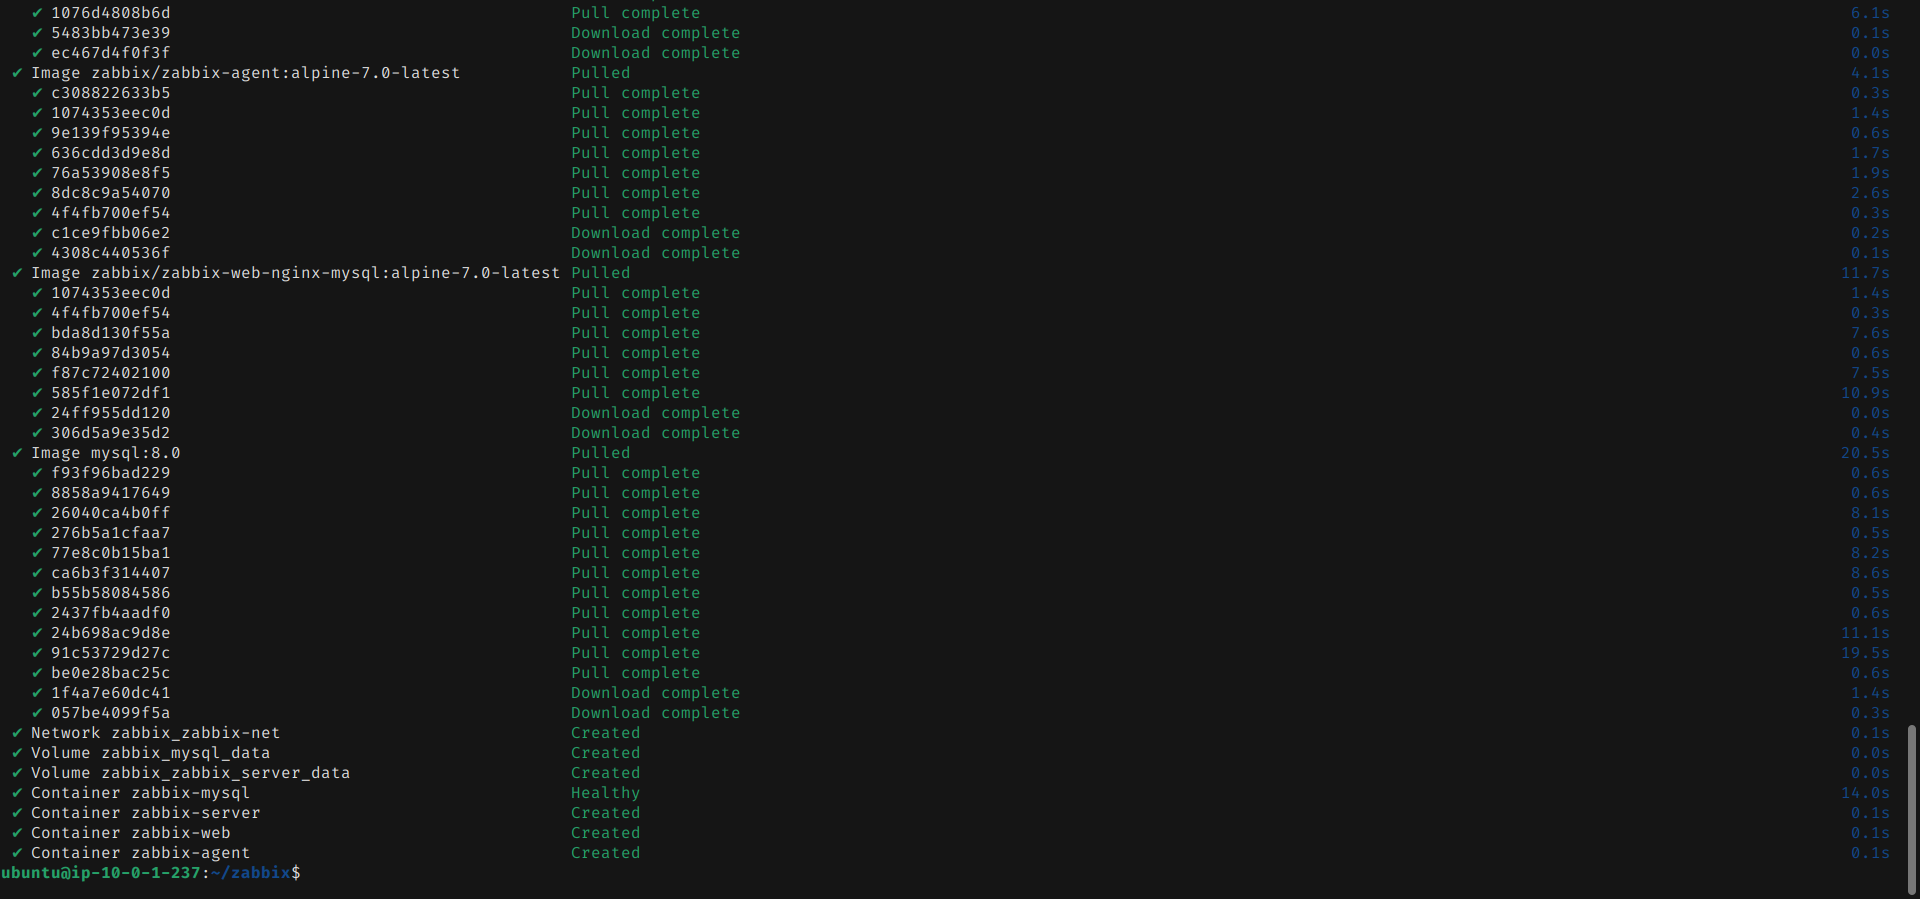
\includegraphics[width=0.95\textwidth]{images/16-docker-compose-up.png}
\caption{Lancement des conteneurs Docker}
\label{fig:docker-compose-up}
\end{figure}

\subsection{Vérification des Conteneurs}

\begin{lstlisting}[language=bash, caption=Vérification de l'état des conteneurs]
docker compose ps
\end{lstlisting}

\begin{figure}[H]
\centering
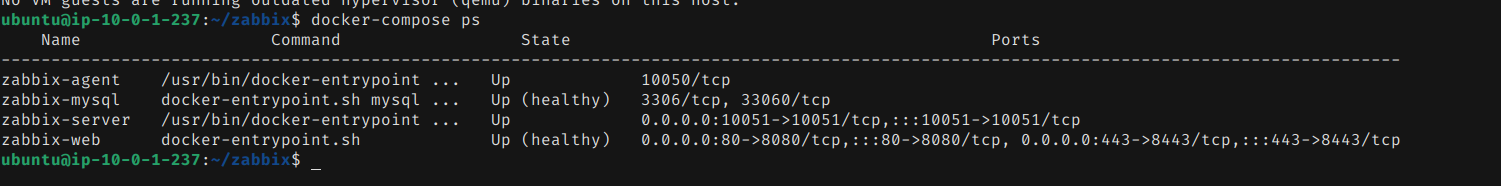
\includegraphics[width=0.95\textwidth]{images/17-containers-running-status.png}
\caption{Conteneurs Zabbix en cours d'exécution}
\label{fig:containers-running}
\end{figure}

Les 4 conteneurs doivent être en état \texttt{running} :
\begin{itemize}
    \item \textbf{zabbix-mysql} : Base de données MySQL 8.0
    \item \textbf{zabbix-server} : Serveur Zabbix 7.0
    \item \textbf{zabbix-web} : Interface Web Nginx
    \item \textbf{zabbix-agent} : Agent local
\end{itemize}

\section{Accès à l'Interface Web}

\subsection{Connexion à Zabbix}

L'interface Web est accessible via l'IP publique du serveur :

\begin{center}
\fbox{\parbox{0.6\textwidth}{
\centering
\textbf{URL :} \texttt{http://<IP-PUBLIQUE>}\\[0.2cm]
\textbf{Utilisateur :} Admin\\
\textbf{Mot de passe :} zabbix
}}
\end{center}

\begin{figure}[H]
\centering
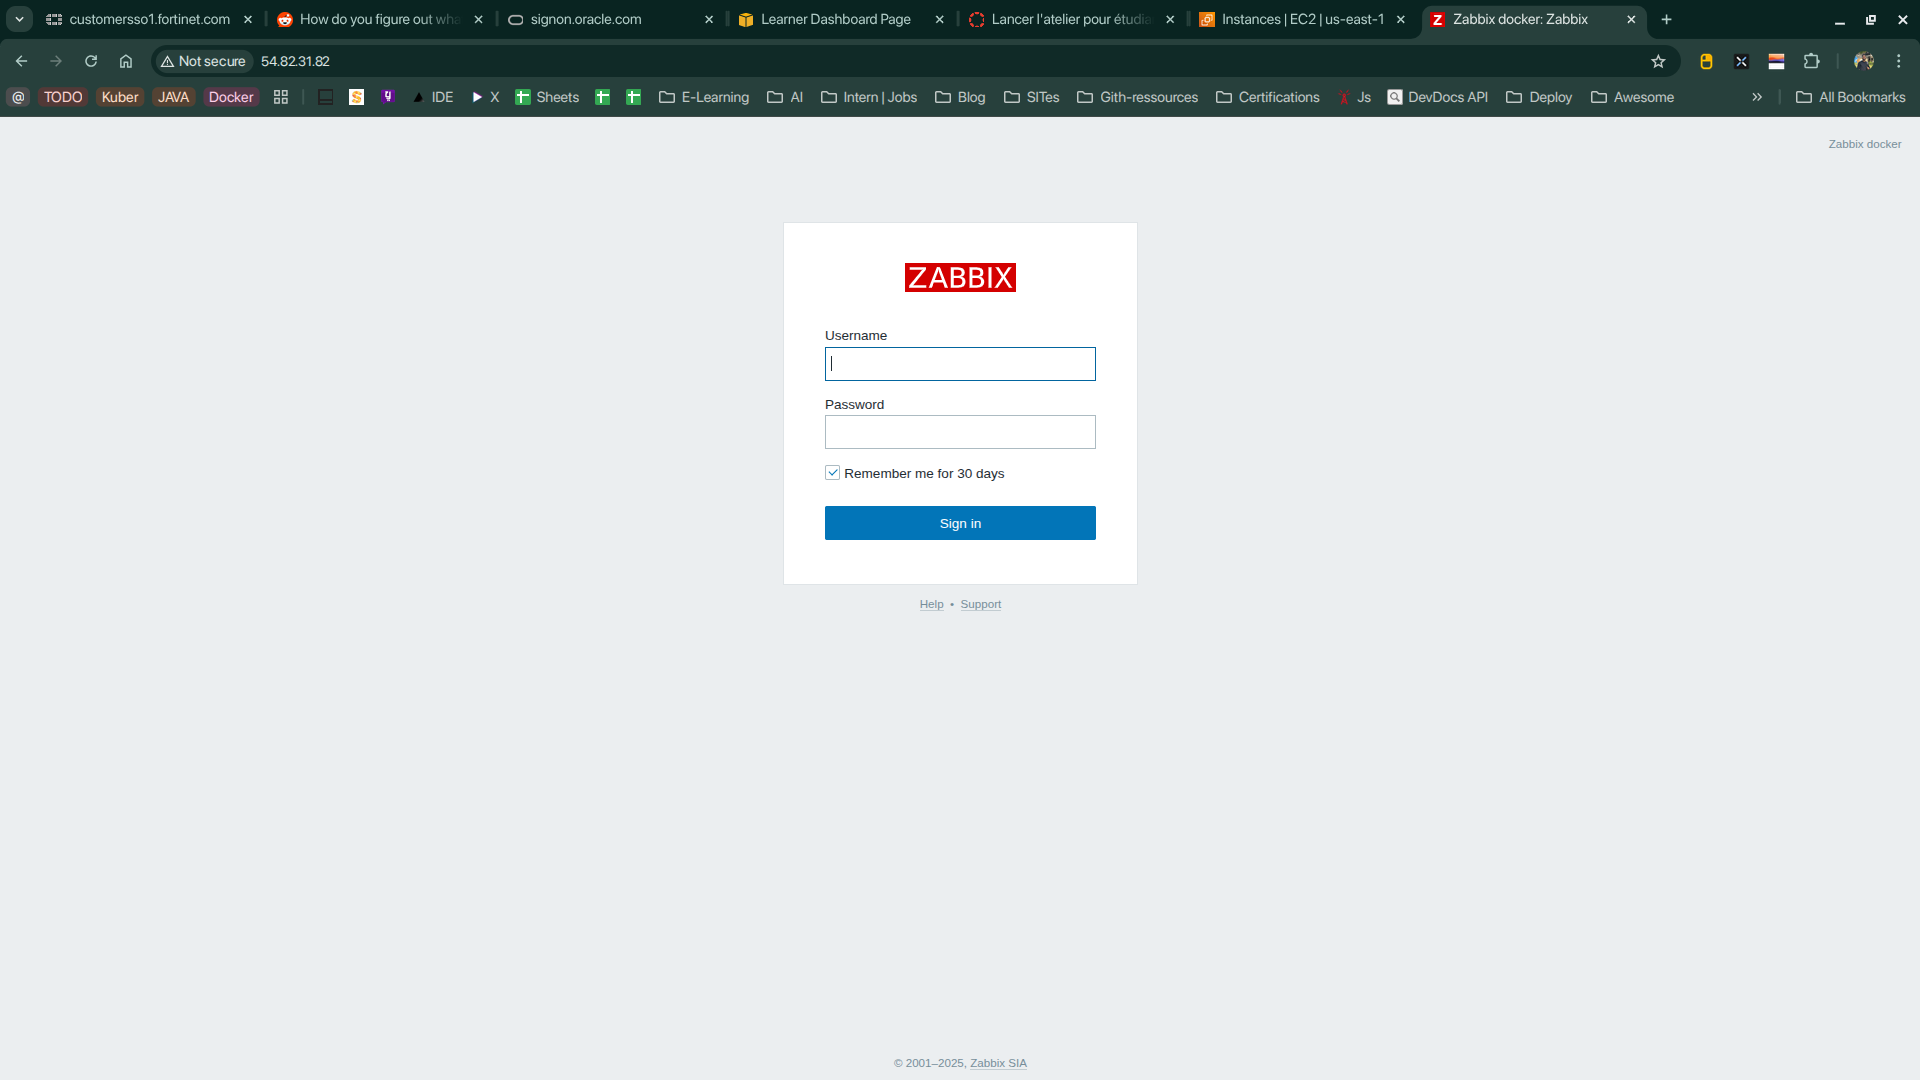
\includegraphics[width=0.85\textwidth]{images/18-zabbix-web-login.png}
\caption{Page de connexion Zabbix}
\label{fig:zabbix-login}
\end{figure}

\subsection{Dashboard Principal}

Après connexion, le tableau de bord principal de Zabbix s'affiche :

\begin{figure}[H]
\centering
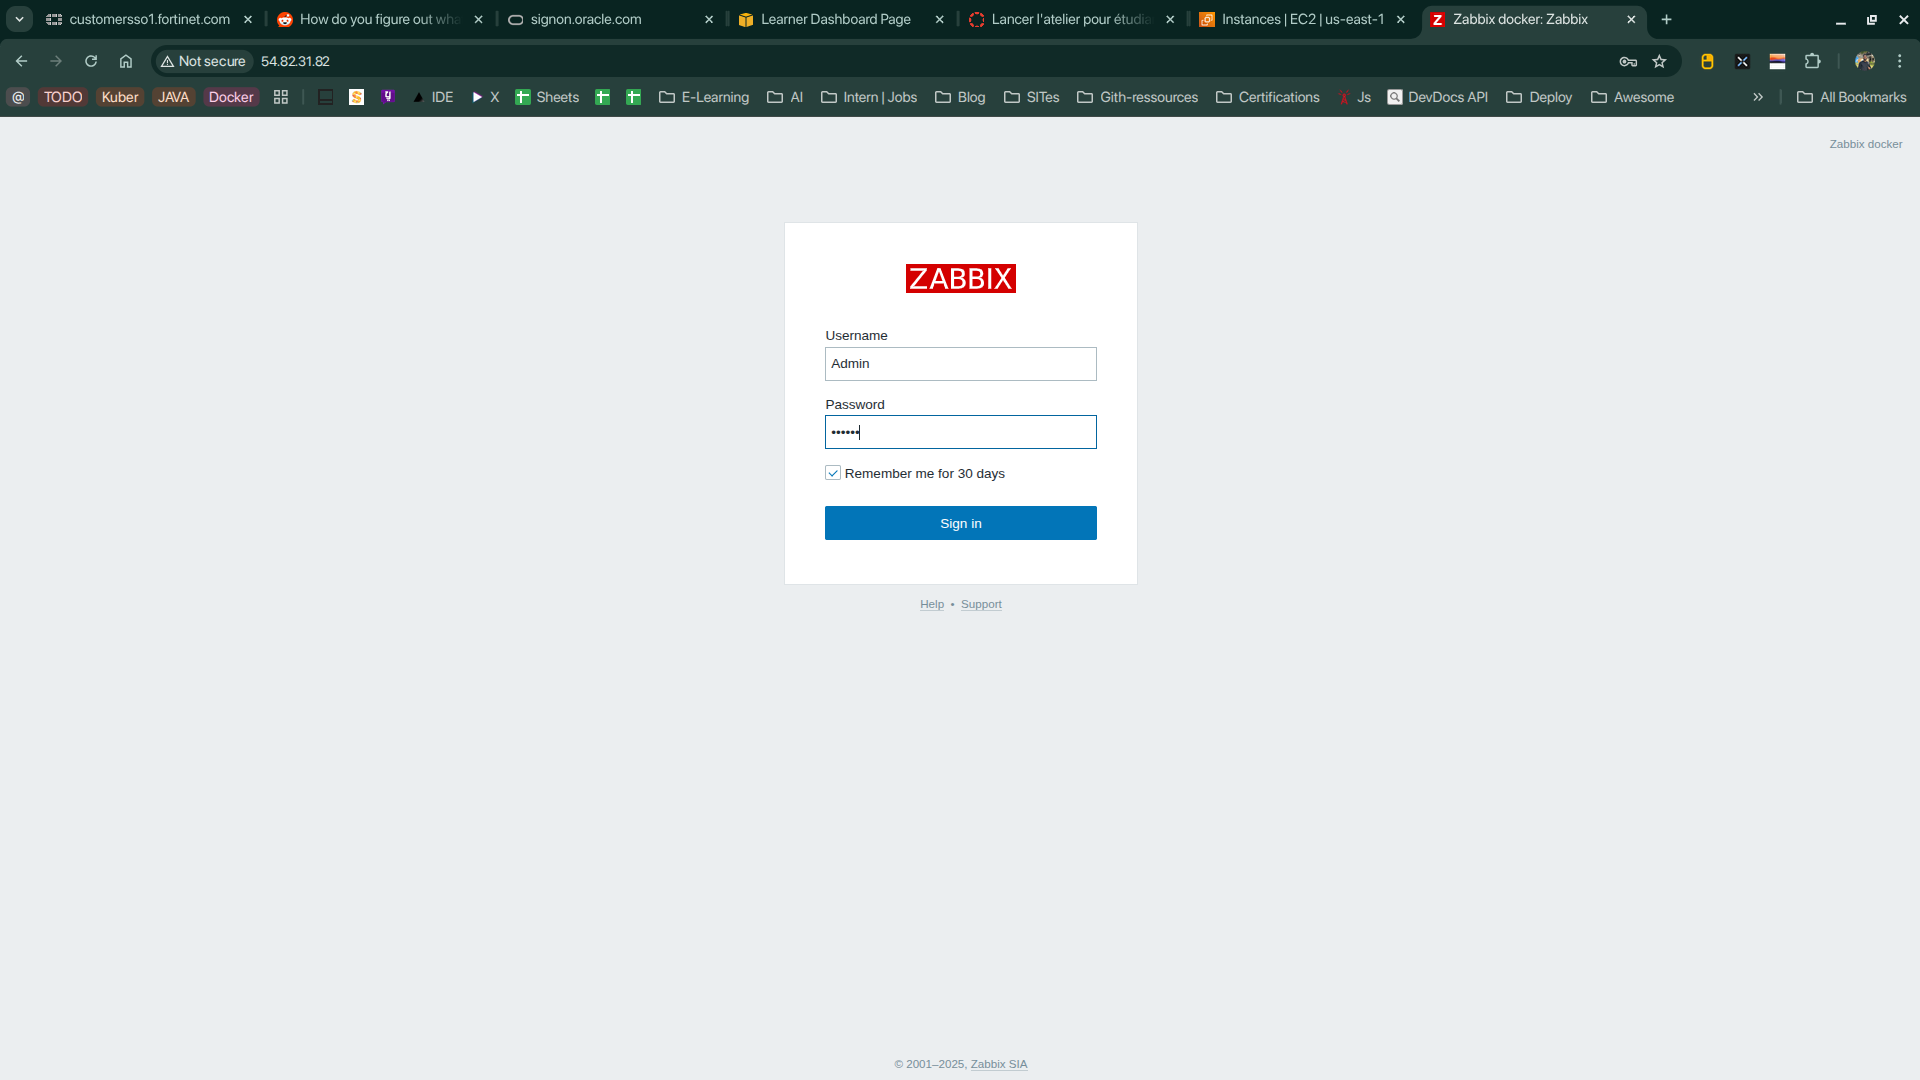
\includegraphics[width=0.95\textwidth]{images/19-zabbix-dashboard.png}
\caption{Dashboard principal de Zabbix}
\label{fig:zabbix-dashboard}
\end{figure}

\section{Architecture des Conteneurs}

\begin{figure}[H]
\centering
\begin{tikzpicture}[
    node distance=1cm,
    container/.style={rectangle, draw=bluecustom, line width=1.5pt, minimum width=3.5cm, minimum height=1cm, align=center, fill=bluecustom!10},
    arrow/.style={->, thick, >=stealth}
]

% Conteneurs
\node[container] (mysql) {MySQL 8.0\\Port 3306};
\node[container, right=2cm of mysql] (server) {Zabbix Server\\Port 10051};
\node[container, right=2cm of server] (web) {Zabbix Web\\Port 80/443};
\node[container, below=1.5cm of server] (agent) {Zabbix Agent\\Port 10050};

% Connexions
\draw[arrow] (server) -- (mysql) node[midway, above] {DB};
\draw[arrow] (web) -- (server) node[midway, above] {API};
\draw[arrow] (agent) -- (server) node[midway, right] {Metrics};

% Network
\node[draw=awsorange, dashed, line width=1pt, fit=(mysql)(server)(web)(agent), inner sep=0.5cm, label={[font=\small]below:zabbix-net (Docker Network)}] {};

\end{tikzpicture}
\caption{Architecture des conteneurs Docker}
\label{fig:docker-architecture}
\end{figure}

\section{Commandes Utiles}

\begin{table}[H]
\centering
\caption{Commandes Docker utiles}
\label{tab:docker-commands}
\begin{tabular}{|l|p{8cm}|}
\hline
\textbf{Commande} & \textbf{Description} \\
\hline
\texttt{docker compose up -d} & Démarrer les conteneurs \\
\hline
\texttt{docker compose down} & Arrêter les conteneurs \\
\hline
\texttt{docker compose ps} & Voir l'état des conteneurs \\
\hline
\texttt{docker compose logs -f} & Voir les logs en temps réel \\
\hline
\texttt{docker compose restart} & Redémarrer tous les conteneurs \\
\hline
\end{tabular}
\end{table}
